% Analyse des pratiques d'encodage des éditions en ligne EHRI

\section{Analyse des pratiques d'encodage}
Avec la publication de plusieurs éditions thématiques, l'équipe d'éditoriale de l'EHRI a pu expérimenter l'utilisation de la TEI et adapter sa pratique. Notre travail a donc débuté par l'observation des pratiques d'encodage des précédentes éditions.  

\subsection{Extraction de l'information}
Le corpus à analyser était composé des quatre éditions, soit un total de trois cent trente-cinq documents. À l'aide d'un \textit{script} Python, nous avons pu extraire toutes les occurrences des balises et attributs utilisés par collection. Nous avons ensuite arrangé les résultats dans un tableau récapitulatif (Annexe \ref{Tableau}).  

\begin{figure}[h]
    \centering
    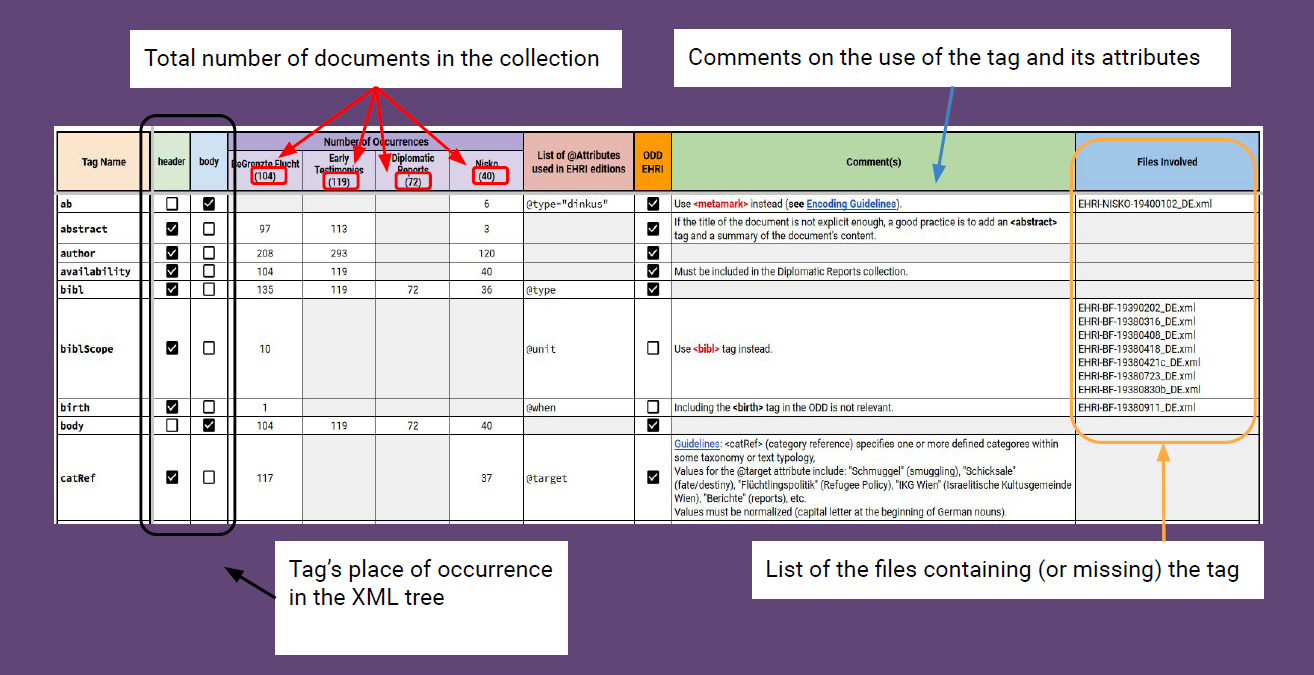
\includegraphics[width=0.95\linewidth]{2-MAIN//images/tableau-fonctionnement.png}
    \caption{Fonctionnement du tableau récapitulatif de l'encodage des éditions EHRI}
    \label{fig:tableau-recap}
\end{figure}  

Les balises sont classées par ordre alphabétique, et une case à cocher permet de voir si la balise se trouve dans le \texttt{<teiHeader>} et/ou dans le \texttt{<body>}. Chaque collection dispose ensuite de sa propre colonne, indiquant pour chaque balise son nombre d'occurrences. Nous avons ensuite établi, pour chaque balise, une liste de tous ses attributs utilisés dans l'encodage EHRI.


\subsection{Évaluation du choix des balises et attributs}
Une fois le tableau récapitulatif en partie rempli, nous avons pu procéder à une analyse plus approfondie de l'encodage. En fonction du contexte, nous avons ajouté des commentaires sur l'utilisation de certaines balises~; une précision sur l'usage recommandé par les \textit{TEI Guidelines} ou une suggestion d'amélioration, par exemple.  

Le tableau a été rendu le plus complet possible grâce à la rédaction d'un \textit{script}, en Python, permettant de rechercher des informations précises dans le corpus (extrait du code en Annexe \ref{Script}). Le nombre d'occurrences de certaines balises a révélé des doublons, à l'instar de la balise \texttt{<creation>}, apparaissant parfois deux fois au sein d'un même fichier. Or, la création d'un document ne peut avoir qu'une seule occurrence. Ce \textit{script} nous a permis de remplir la dernière colonne du tableau, \enquote{\textit{Files Involved}}, pour que les éditeur$\cdot$ice$\cdot$s puissent corriger ce type d'erreurs.



\section{Identification des améliorations possibles}
Le tableau complet donne une bonne vue d'ensemble de l'encodage des éditions EHRI, et notamment de leur évolution. Nous avons identifié deux pistes d'améliorations significatives~: une meilleure conformité aux recommandations de la TEI et l'uniformisation des éditions déjà publiées.  

\subsection{Amélioration de la conformité}
Pour être conforme au standard TEI, un fichier XML doit être bien formé, c'est-à-dire rédigé avec une syntaxe correcte. Le fichier XML doit également être valide. Pour cela, il faut que l'encodage respecte les règles du schéma qui lui a été associé. Enfin, le projet d'encodage doit être renseigné de façon exhaustive dans une ODD\footnote{Nous aborderons la notion d'ODD dans le chapitre suivant.} (\enquote{\textit{One Document Does-it all}}), elle aussi conforme.  

Parmi les bonnes pratiques que nous recommandons dans le traitement d'un corpus comme celui des éditions EHRI, il y a tout d'abord la question de l'identifiant du fichier. Les fichiers EHRI portent tous un identifiant unique basé sur une même structure~: \enquote{\texttt{EHRI-<collection>-YYYYMMDD\_{}<langue>}} (par exemple, \enquote{\texttt{EHRI-BF-19380315\_{}DE}}). Cet identifiant doit être la valeur de l'attribut \texttt{@xml:id} qui se trouve dans la balise ouvrante de l'élément racine \texttt{<TEI>}.  

Le seconde recommandation qui nous paraît particulièrement importante est la structuration du contenu à l'intérieur de la balise \texttt{<body>}. Pour assurer un bon affichage du contenu et éviter la multiplication inutile de fichiers, nous proposons d'encoder la transcription du fac-similé et ses traductions au sein d'un même fichier. Il y aurait donc au moins une division \texttt{<div>} de premier niveau, complétée par un attribut \texttt{@type} dont la valeur serait \texttt{"transcription"} ou \texttt{"translation"}. Dans le cas des traductions, l'attribut \texttt{@xml:lang} apporterait une précision sur la langue de la traduction contenue dans la division.


\subsection{Uniformisation des édition}

\subsubsection{Utilisation de l'anglais}
La nature européenne du projet EHRI implique que les différents acteurs ne parlent pas tous la même langue. La langue la plus communément parlée parmi les éditeur$\cdot$ice$\cdot$s et le public des éditions est l'anglais. Il nous paraît donc logique de normaliser l'utilisation de l'anglais comme langue d'encodage des métadonnées et de la valeur des attributs. Cela permet à quiconque accédant aux fichiers XML d'en comprendre l'encodage. Nous avons ainsi parfois été confronté$\cdot$e à des valeurs d'attributs en allemand. Le problème posé par l'utilisation de l'allemand pour préciser la valeur des attributs est le risque d'une perte sémantique lors de sa traduction dans une autre langue. Or, les valeurs d'attributs proposées par les \textit{TEI Guidelines} dans leur documentation d'éléments sont toujours en anglais, ce qui facilite le travail d'encodage et la réutilisation du schéma produit pour l'édition.

\subsubsection{Standardisation de la valeur de certains attributs}
Il est essentiel que les valeurs des attributs soient uniformes. Pour certains attributs, il existe des normes que l'on peut choisir d'appliquer. Par exemple, il existe une norme d'encodage concernant le format des dates~: l'utilisation de l'attribut \texttt{@when-iso} sera privilégié si la date est au format \enquote{\texttt{YYYY-MM-DD}} (norme ISO 8601\footnote{Récapitulatif de la norme ISO 8601 sur Wikipédia~: \texttt{\href{https://fr.wikipedia.org/wiki/ISO_8601}{https://fr.wikipedia.org/wiki/ISO\_{}8601}} (visité le 03/09/2023).}), sinon on lui préférera l'attribut \texttt{@when}. Cela est d'autant plus important qu'une date incomplète avec un attribut \texttt{@when-iso} causera un bug d'affichage, et qu'une date complète avec un attribut \texttt{@when} ne s'affichera pas correctement. Il n'existe, en revanche, pas de normes concernant l'attribut \texttt{@type}, ses valeurs possibles étant aussi variées que la diversité des éléments auquel il peut être associé.  

L'importance de la valeur de l'attribut \texttt{@xml:lang} peut paraître abstraite. En général, et même s'il est possible d'écrire le nom de la langue en toutes lettres, nous utilisons un code pour donner la valeur de l'attribut de langue. Or, ce code doit s'inscrire dans un système établi~: c'est le rôle des normes. Prenons l'exemple de la langue allemande~: \enquote{Allemand} en français, \enquote{\textit{German}} en anglais, et \enquote{\textit{Deutsch}} en allemand. Sans système pré-établi, l'éditeur$\cdot$ice sera naturellement tenté$\cdot$e d'utiliser un code parlant pour sa propre langue. Nous obtiendrions donc les possibilités suivantes~: \enquote{\texttt{"all"}}, \enquote{\texttt{"ger"}} et \enquote{\texttt{"deu"}} respectivement. Le problème devient évident. Le choix ne peut pas revenir à l'éditeur$\cdot$ice de déterminer lui$\cdot$elle-même des codes à utiliser. Il existe en outre des préférences, qui ne regardent que les traducteur$\cdot$ice$\cdot$s, concernant le choix de traduire certains termes ou de les laisser apparaître dans leur langue originale. Ce problème s'applique également ici.  

Plusieurs systèmes existent. La norme ISO 639\footnote{Récapitulatif de la norme ISO 639 sur Wikipédia~: \texttt{\href{https://fr.wikipedia.org/wiki/ISO_639}{https://fr.wikipedia.org/wiki/ISO\_{}639}} (visité le 03/09/2023).} définit des codes pour les langues à deux ou trois caractères (ISO 639-1 ou ISO 639-2). Le problème posé par cette norme est qu'elle ne tranche pas entre l'utilisation de deux ou trois caractères, ce qui peut conduire à une certaine confusion. Nous avons donc opté pour le registre de codes établi par l'Iana\footnote{\enquote{\textit{Iana Language Subtag Registry}}~: \texttt{\href{https://www.iana.org/assignments/language-subtag-registry/language-subtag-registry}{https://www.iana.org/assignments/language-subtag- registry/language-subtag-registry}}.}. Celui-ci a l'avantage de ne proposer qu'une norme, précise et très régulièrement mise à jour. 